\section{Experiments}
\subsection{Experimental Setup}
\par To evaluate our detection attack, we run multiple Bitcoin clients on different virtual machines in Univerity of Massachuset campus network. Each virtual machine is connected to the Internet with high bandwidth. Bitcoin clients are connected to the Bitcoin network for a while and as a result the block-chain ledger is updated. We capture Bitcoin traffic for from ... to ... . 
\par In our threat model we are assuming that our traffic is passing through a VPN or any tunnel which encrypt the traffic and may include other traffics than Bitcoin traffic. To model the background traffic we use CAIDA anonymized traces which we will discuss in the next section. 

\subsection{Modeling Background Traffic}
To model background traffic we use CAIDA anonymized traces. We separate traffic flow of each IP address and define each flow as traffic of one user. The traffic length of each user is 1 hour. To have traffic with different length we concat traffic of different users. Also, to model different background traffic intensity we sum up traffic flow of different users' flow. 
\subsubsection{Tor Background Traffic}
\par To model background traffic behind Tor, we capture traffic of 1000 different website behind Tor in the conditions that only one tab is open. To model different noise intensity we assume that the user has opened multiple tabs at the same time. 

\subsection{Detection Scheme's Threshold}
\shahrzad{
\begin{itemize}
\item  showing the correlation value against ground-truth and ground-false and showing they are distinguishable
\item  discussing different thresholds and comparing them
\end{itemize} }


\subsection{Impact of Background Traffic}
\par When Bitcoin traffic doesn't have any background traffic, it will have a very high correlation with block-chain time trace. As we discuss in our threat model, Bitcoin traffic will aggregate with other types of traffic. In this section we investigate background traffic impact on our both detection scheme. Figure \ref{fig:window_effect_users} shows true positive and false positive of our window-based correlation scheme and figure \ref{fig:stat_effect_users} shows the true positive and false positive of the statistical scheme. 
\par By comparing figure \ref{fig:window_effect_users} and \ref{fig:stat_effect_users} we can see the detection scheme of window-based scheme is far better. However, in the recent update of Bitcoin in January 2017, compact blocks are introduced, which the window-based correlation scheme true positive drop dramatically. In section \ref{sec:compactblock} we discuss compact block detection mechanism thoroughly. 
\begin{figure}
\centering
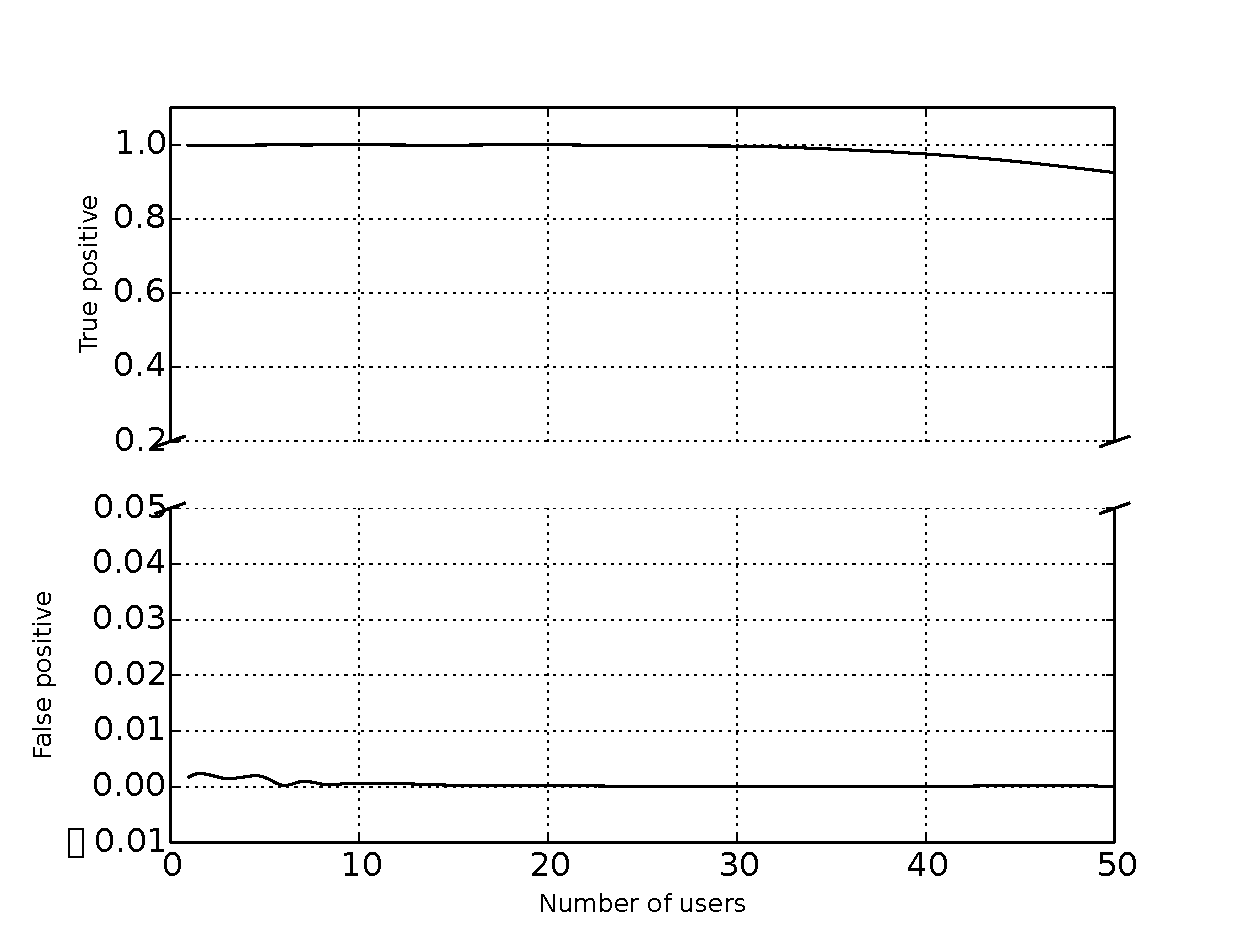
\includegraphics[scale=0.4]{image/window_effect_users.eps}
\caption{True positive and False positive of detecting traffic traces including Bitcoin and different number of users using window-based correlation scheme}
\label{fig:window_effect_users}
\end{figure}

\begin{figure}
\centering
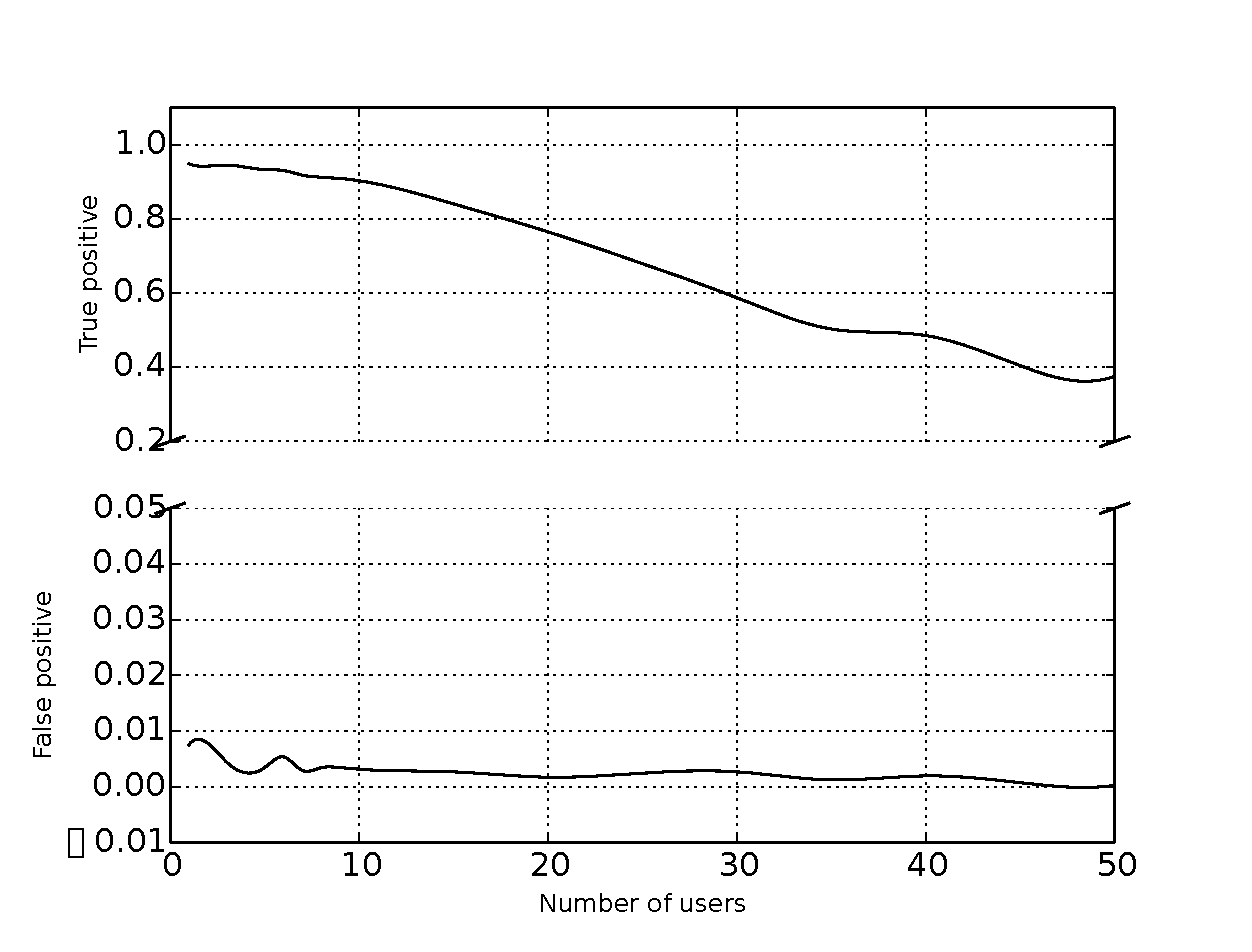
\includegraphics[scale=0.4]{image/stat_effect_users.eps}
\caption{True positive and False positive of detecting traffic traces including Bitcoin and different number of users using statistical correlation scheme}
\label{fig:stat_effect_users}
\end{figure}
\subsection{Impact of Captured Traffic Length}
The other factor that has impact on the true positive and false positive on our both detection scheme is the length of captured bitcoin traffic. Figure \ref{} and \ref{fig:stat_effect_length} shows this impact for window-based and statistical  correlation scheme respectively when the traffic consist of 1 bitcoin user and 5 other type of traffic users. \shahrzad{figure window-based will be added:Running experiment}
\par According to the figure \ref{fig:stat_effect_length} by having a traffic length more than 20 hours we could achieve good true positive and low false positive. 
\begin{figure}
\centering
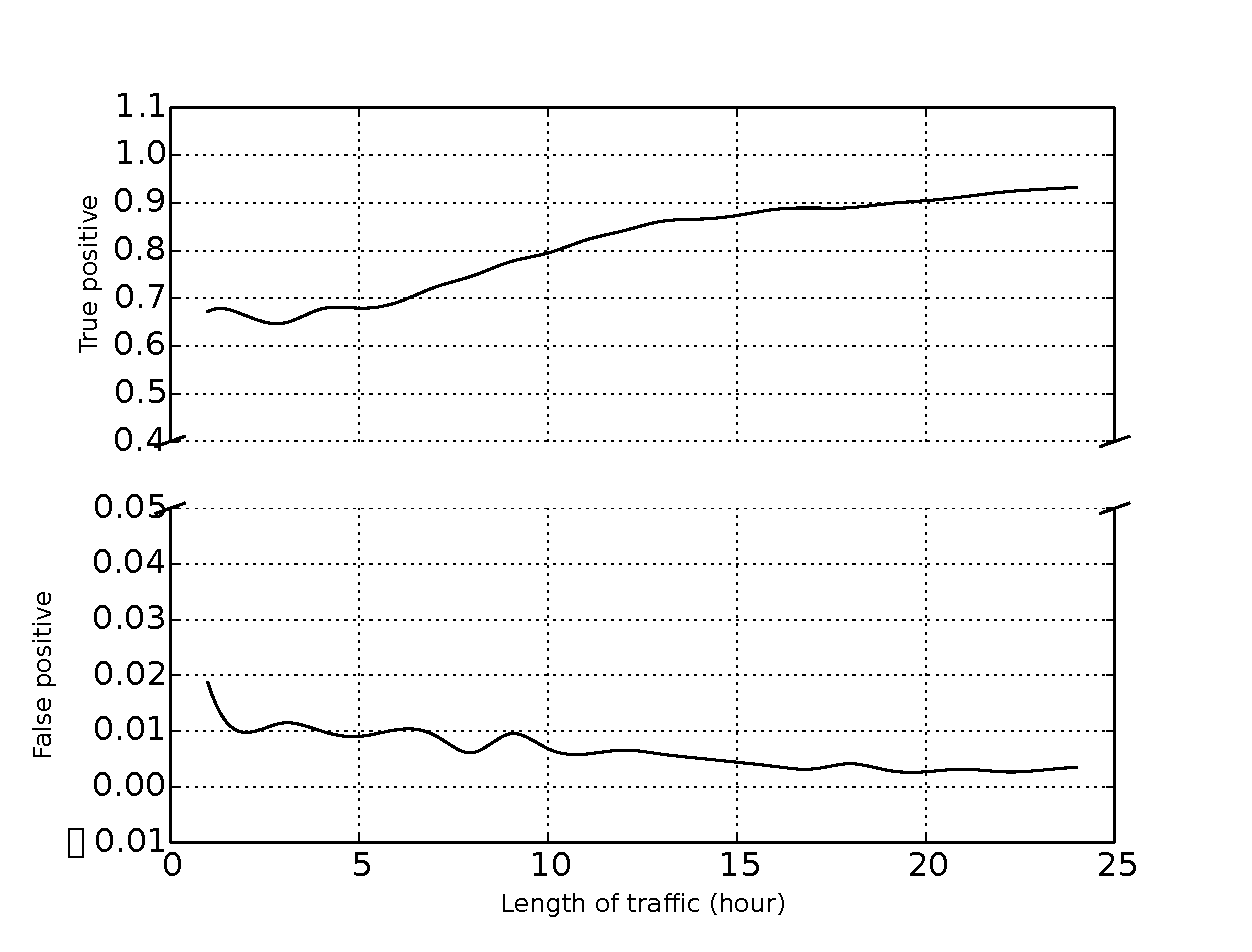
\includegraphics[scale=0.4]{image/stat_effect_length.eps}
\caption{True positive and False positive of Bitcoin detection scheme using statistical scheme. The traffic trace consist of 1 Bitcoin user and 5 other users.}
\label{fig:stat_effect_length}
\end{figure}

\subsection{Impact of User's Bandwidth}
As we can see in figure \ref{fig:stat_effect_bw} and \ref{fig:window_effect_bw} bandwidth has impact on both statistical correlation scheme and window-based correlation scheme. \shahrzad{TBW}
\begin{figure}
\centering
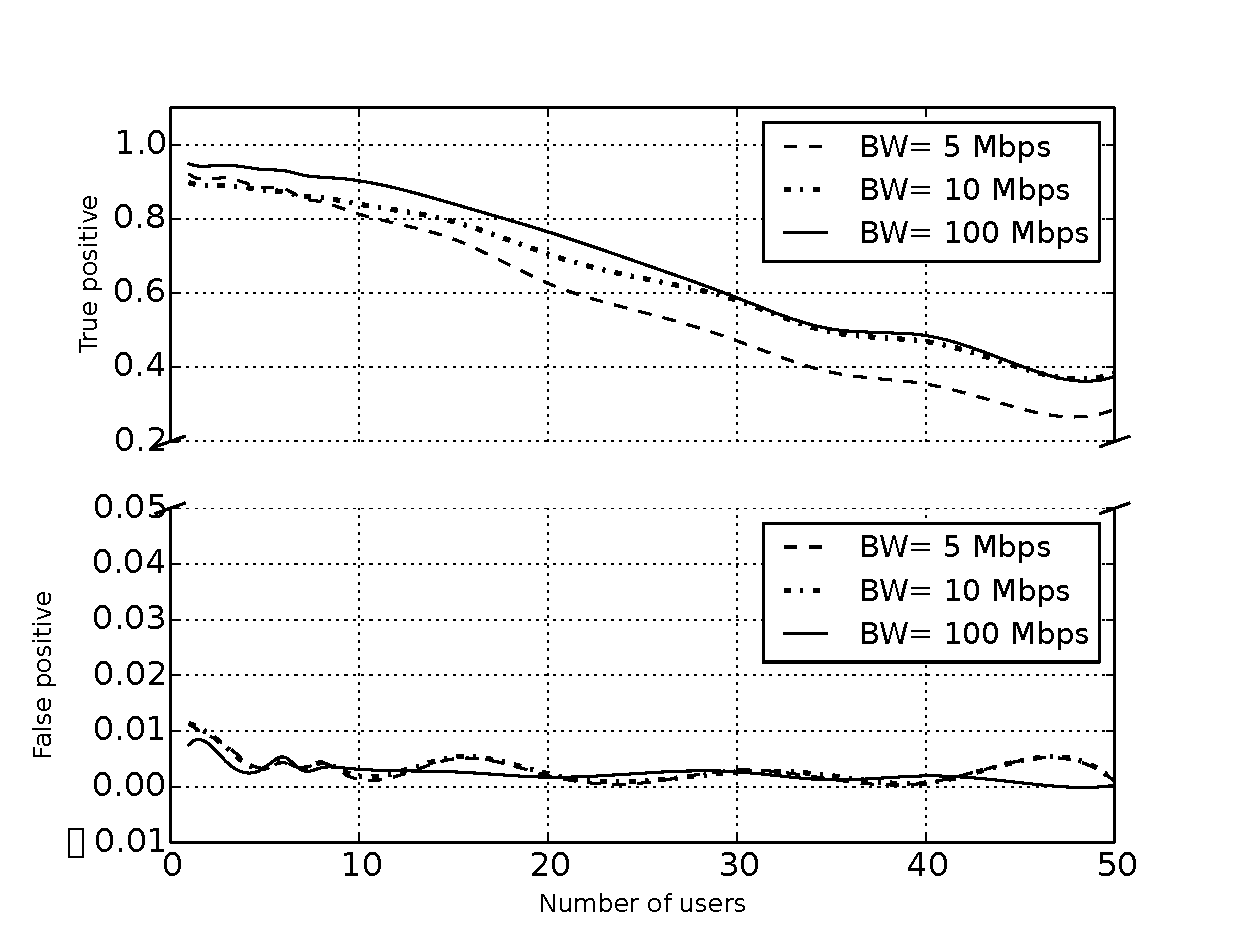
\includegraphics[scale=0.4]{image/stat_effect_bw.eps}
\caption{Effect of bandwidth on the true positive and false positive of detection using statistical correlation scheme. Length of captured traffic is 24 hour.}
\label{fig:stat_effect_bw}
\end{figure}

\begin{figure}
\centering
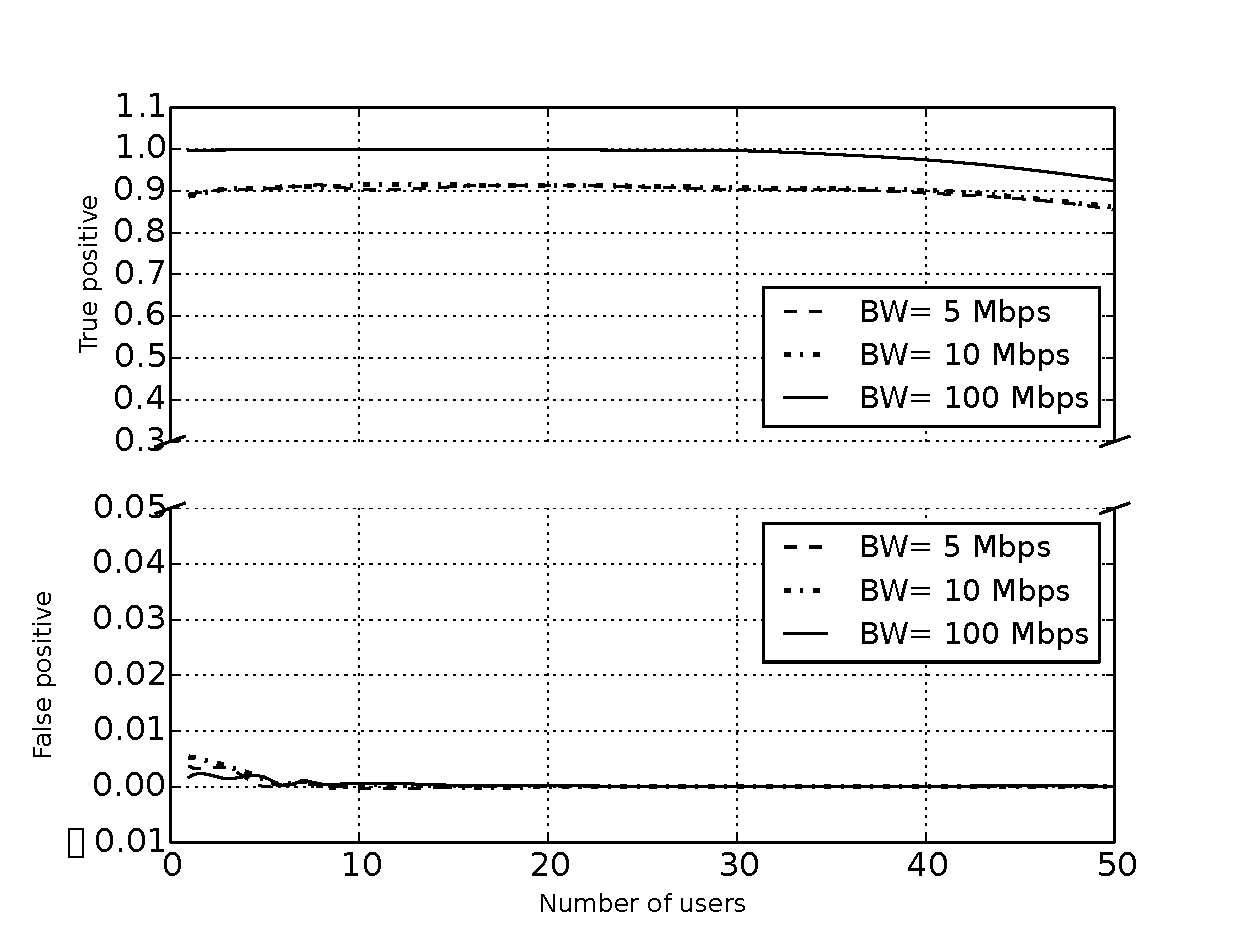
\includegraphics[scale=0.4]{image/window_effect_bw.eps}
\caption{Effect of bandwidth on the true positive and false positive of detection using  window-based correlation scheme. Length of captured traffic is 24 hour.}
\label{fig:window_effect_bw}
\end{figure}

\subsection{Bitcoin Behind Tor}
As we can see in the figure \ref{fig:stat_effect_tor} running Bitcoin behind Tor, doesn't hide the fact that the user is using Bitcoin. And we still detect using Bitcoin when the user has low background traffic intensity. This is due to the fact that packet delay in Tor usually is less than 1 second, however the traffic volume that we are looking to is volume of 60 seconds interval. 
\begin{figure}
\centering
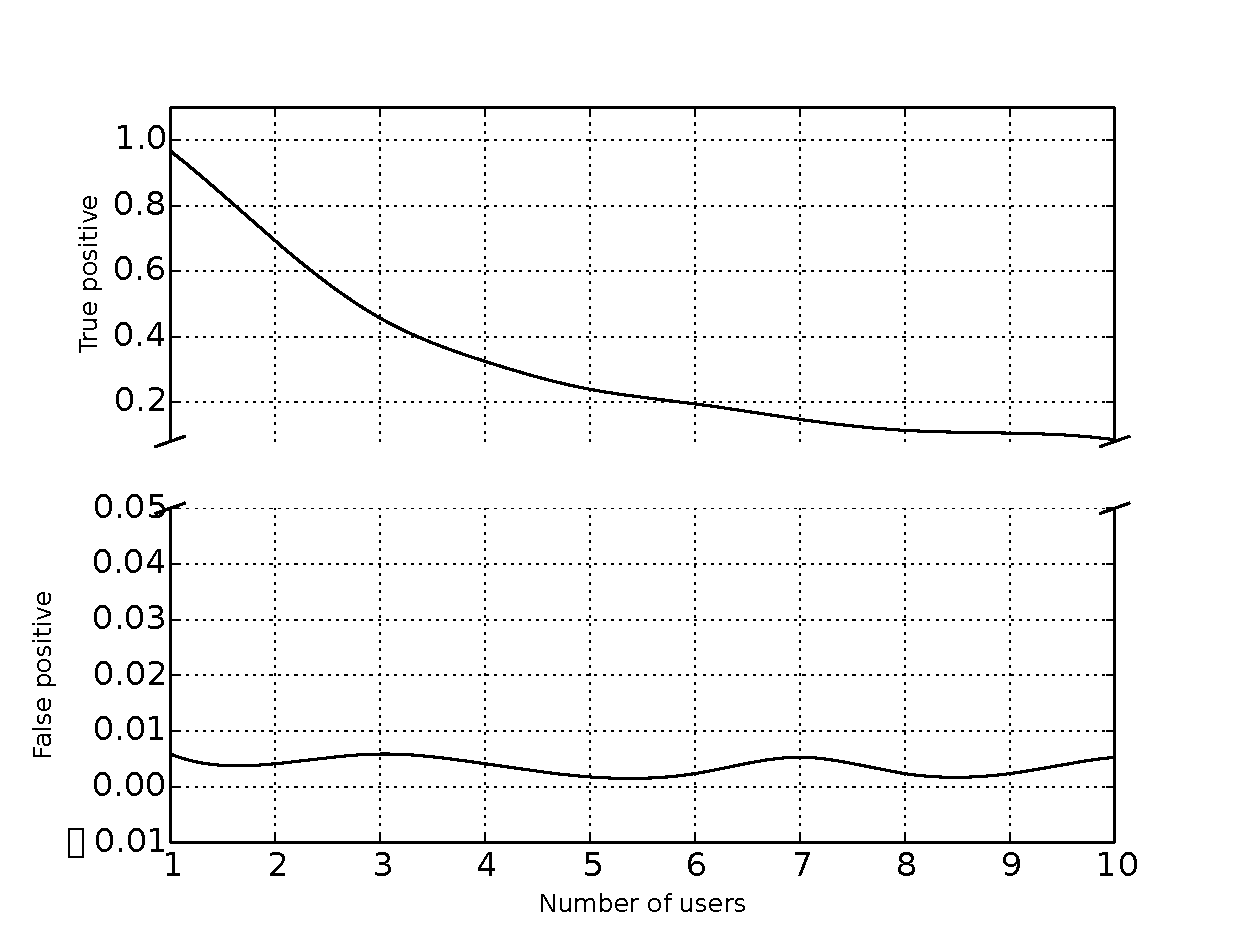
\includegraphics[scale=0.4]{image/stat_effect_tor.eps}
\caption{True positive and false positive of detection of Bitcoin user behind Tor using statistical correlation scheme. Length of traffic is 24 hour.}
\label{fig:stat_effect_tor}
\end{figure}

\subsection{Compact Blocks}\label{sec:compactblock}
\subsubsection{Propagation delay}
Figure \ref{fig:cmpctblock_time_difference} shows the propagation delay in the compact block version of Bitcoin. 
\begin{figure}
\centering
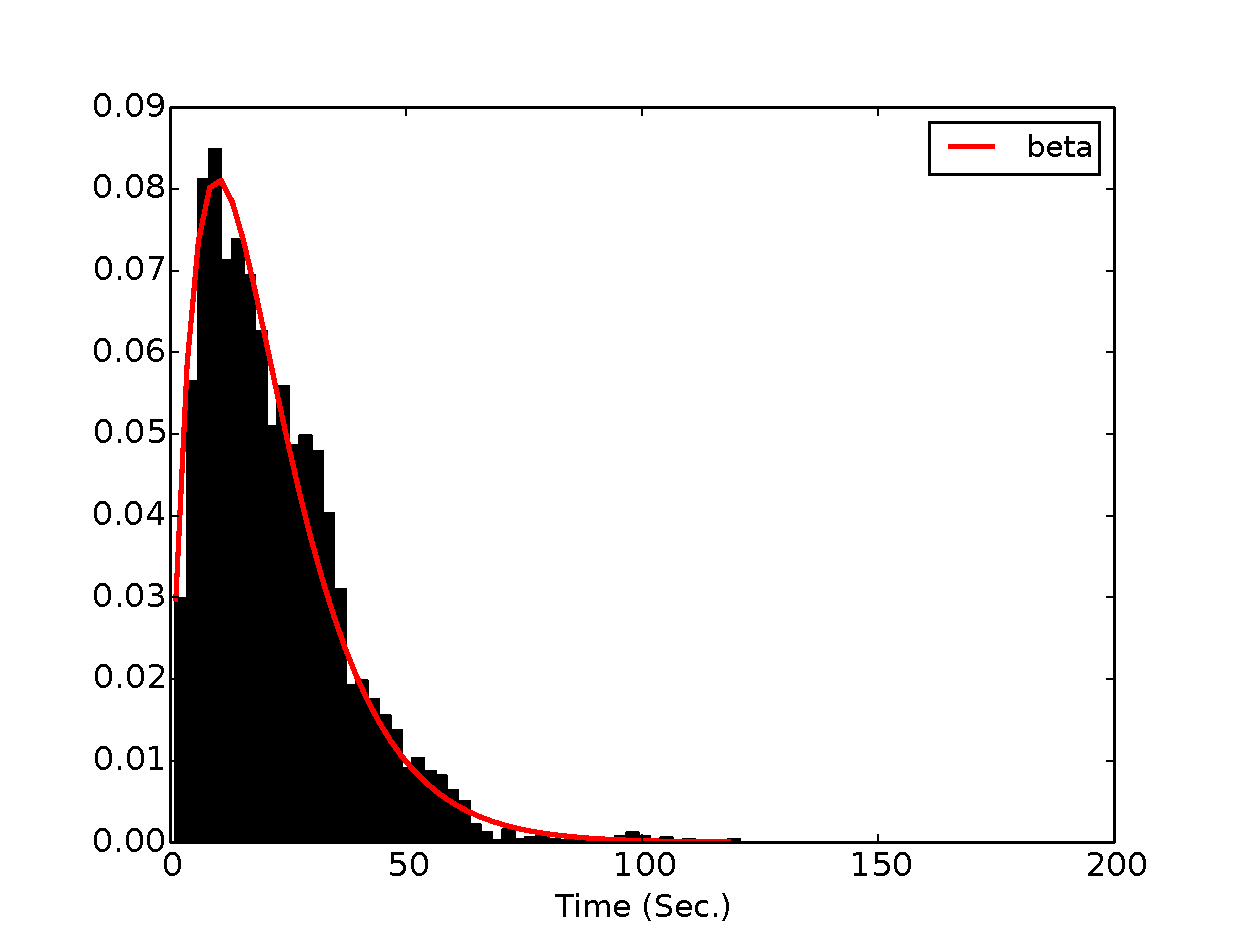
\includegraphics[scale=0.4]{image/cmpctblock_time_difference.eps}
\caption{}
\label{fig:cmpctblock_time_difference}
\end{figure}
\subsubsection{Traffic Pattern}
\shahrzad{Figure \ref{fig:cmpctblock_traffic_volume_detectable} shows the traffic of Bitcoin in the compact block mode which still we can detect positions of blocks. However, figure \ref{fig:cmpctblock_traffic_volume_undetectable} the volume of incoming blocks are not detectable from the other traffics. }
\begin{figure}
\centering
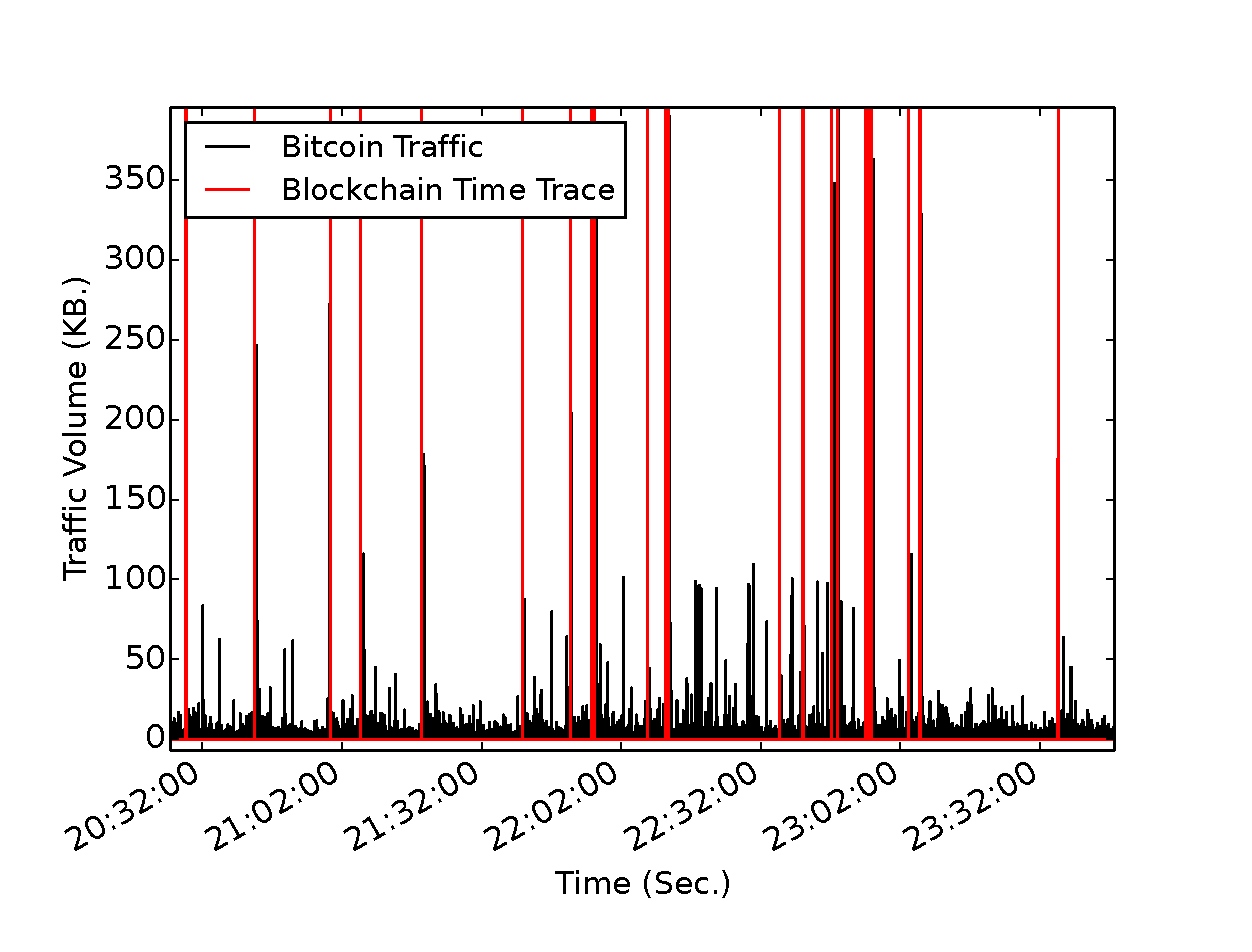
\includegraphics[scale=0.4]{image/cmpctblock_traffic_volume_good.eps}
\caption{}
\label{fig:cmpctblock_traffic_volume_detectable}
\end{figure}

\begin{figure}
\centering
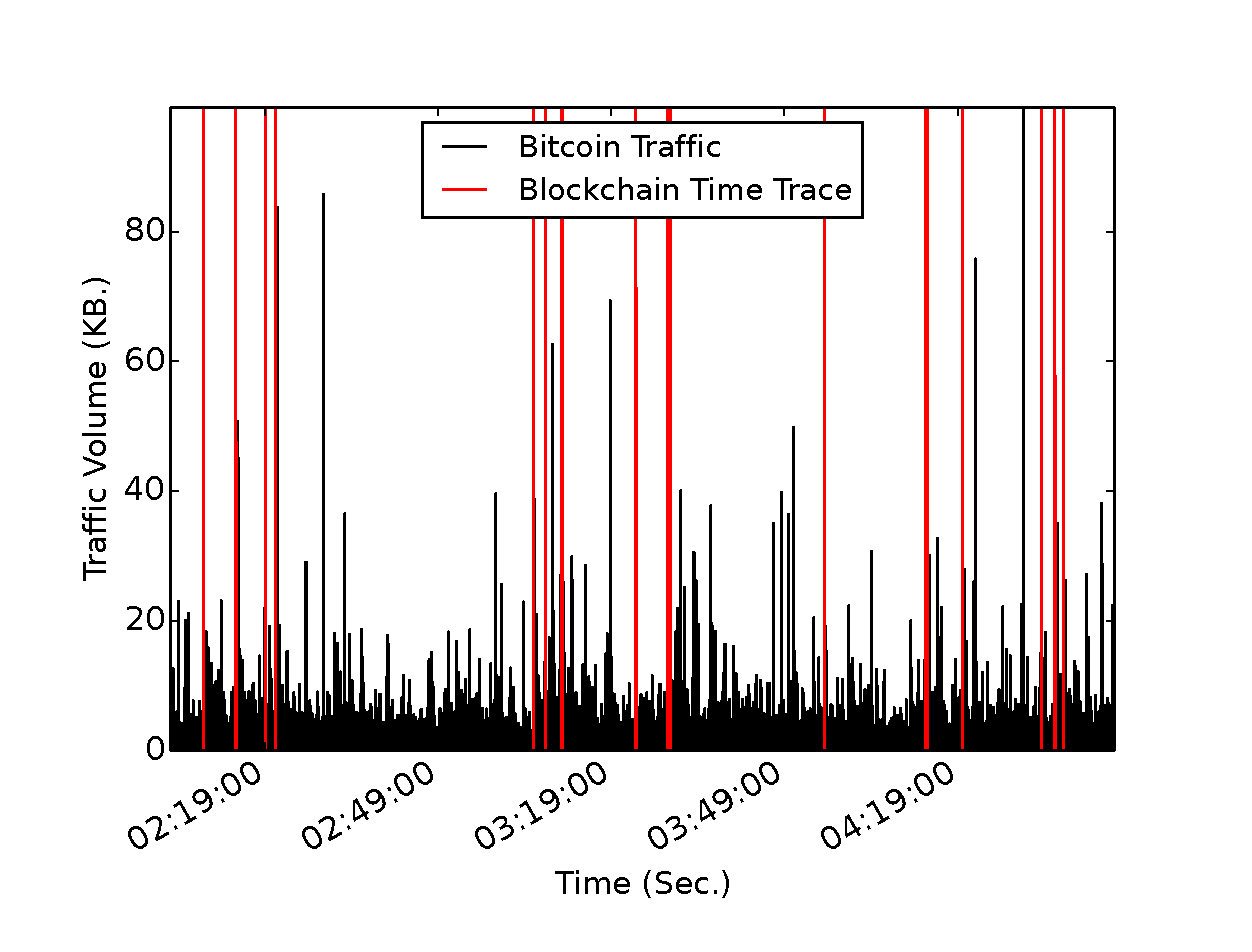
\includegraphics[scale=0.4]{image/cmpctblock_traffic_volume_bad.eps}
\caption{}
\label{fig:cmpctblock_traffic_volume_undetectable}
\end{figure}

\subsubsection{\code{blocktxn} Message}
Figure \ref{fig:blocktxn_volume} shows the amount of blocks volume which is transmitted with \code{blocktx} message. Also figure \ref{fig:blocktxn_time_difference} shows the duration of time which take to download the the rest of the block via \code{blocktxn} message. 

\begin{figure}
\centering
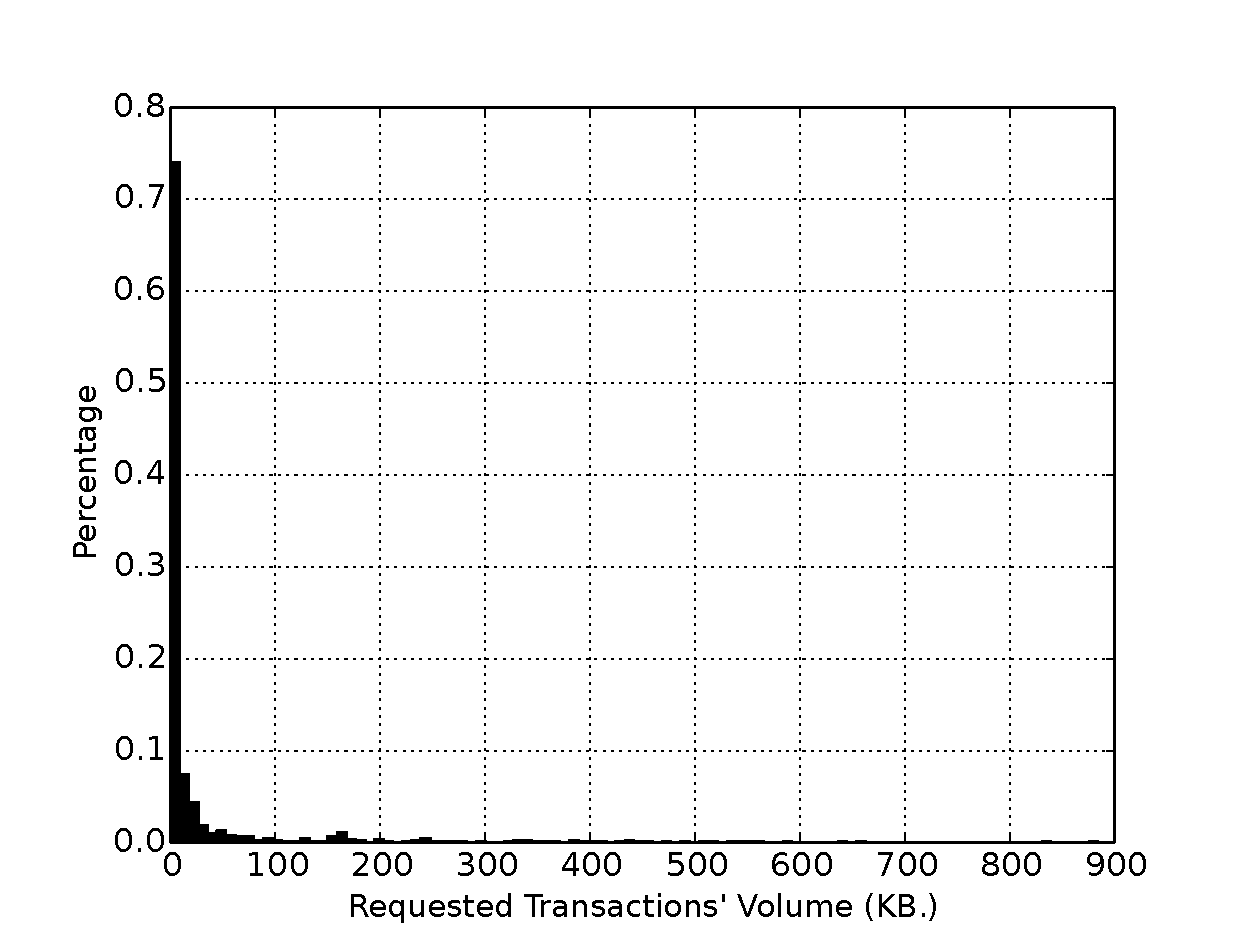
\includegraphics[scale=0.4]{image/blocktxn_volume.eps}
\caption{}
\label{fig:blocktxn_volume}
\end{figure}

\begin{figure}
\centering
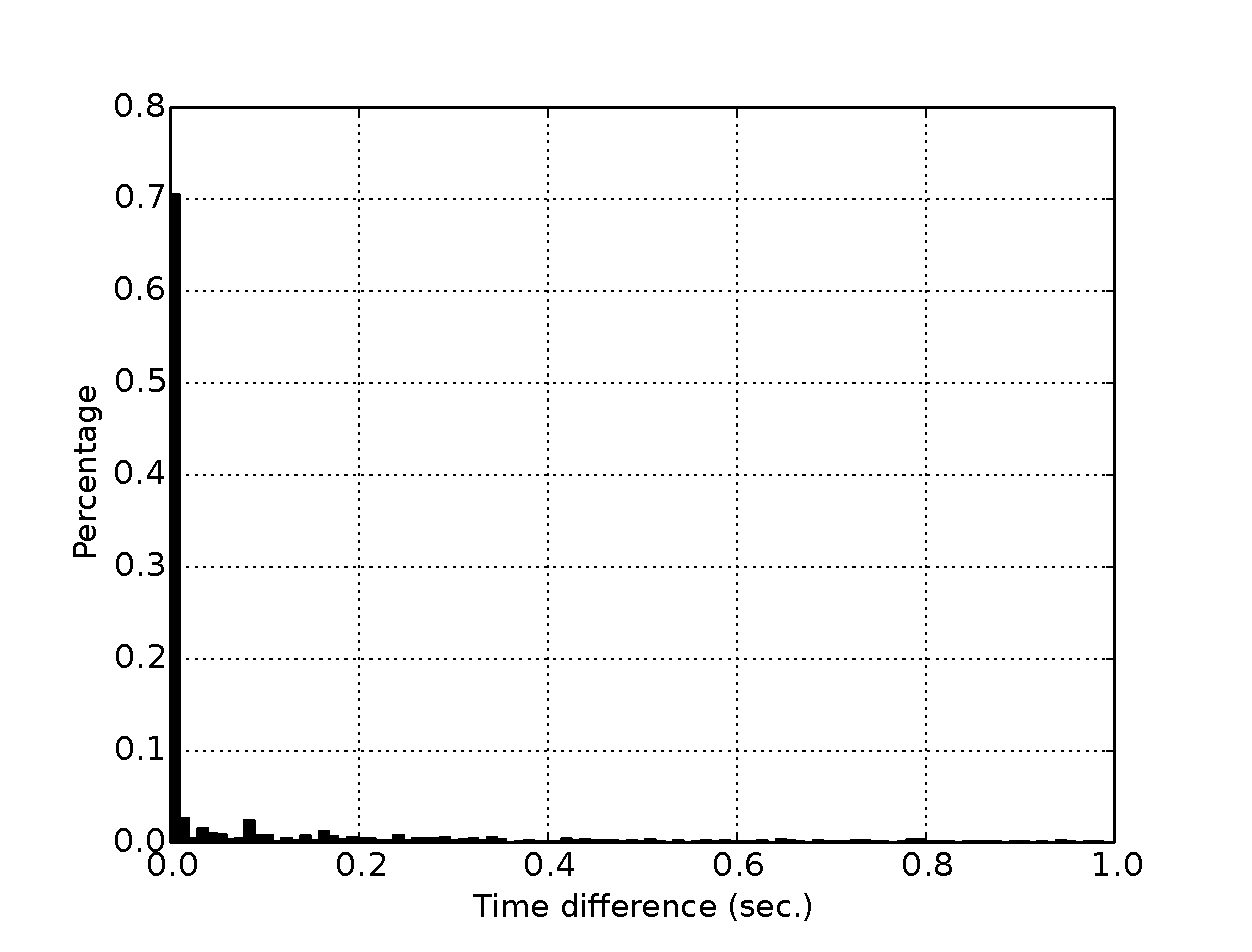
\includegraphics[scale=0.4]{image/blocktxn_time_difference.eps}
\caption{}
\label{fig:blocktxn_time_difference}
\end{figure}


\subsubsection{Traffic Volume Analysis}
In the compact blocks proposal, the peers send sketches of the blocks to receiving peers. This sketches is consist of header of new block, shortened transaction identifiers, and some full transaction which the sending peer predicts the receiving peer doesn't have yet~\cite{compactblock}. Size of new block's header is 80 byte and the shortened transaction identifiers are 6 bytes.  We empirically evaluate a range for the volume size of full transaction which are sent to the receiving peer. Figure \ref{fig:cmpctblock_traffic_volume} shows the volume sizes of blocks sent after \code{cmpctblock} in 1 second. 
\begin{figure}
\centering
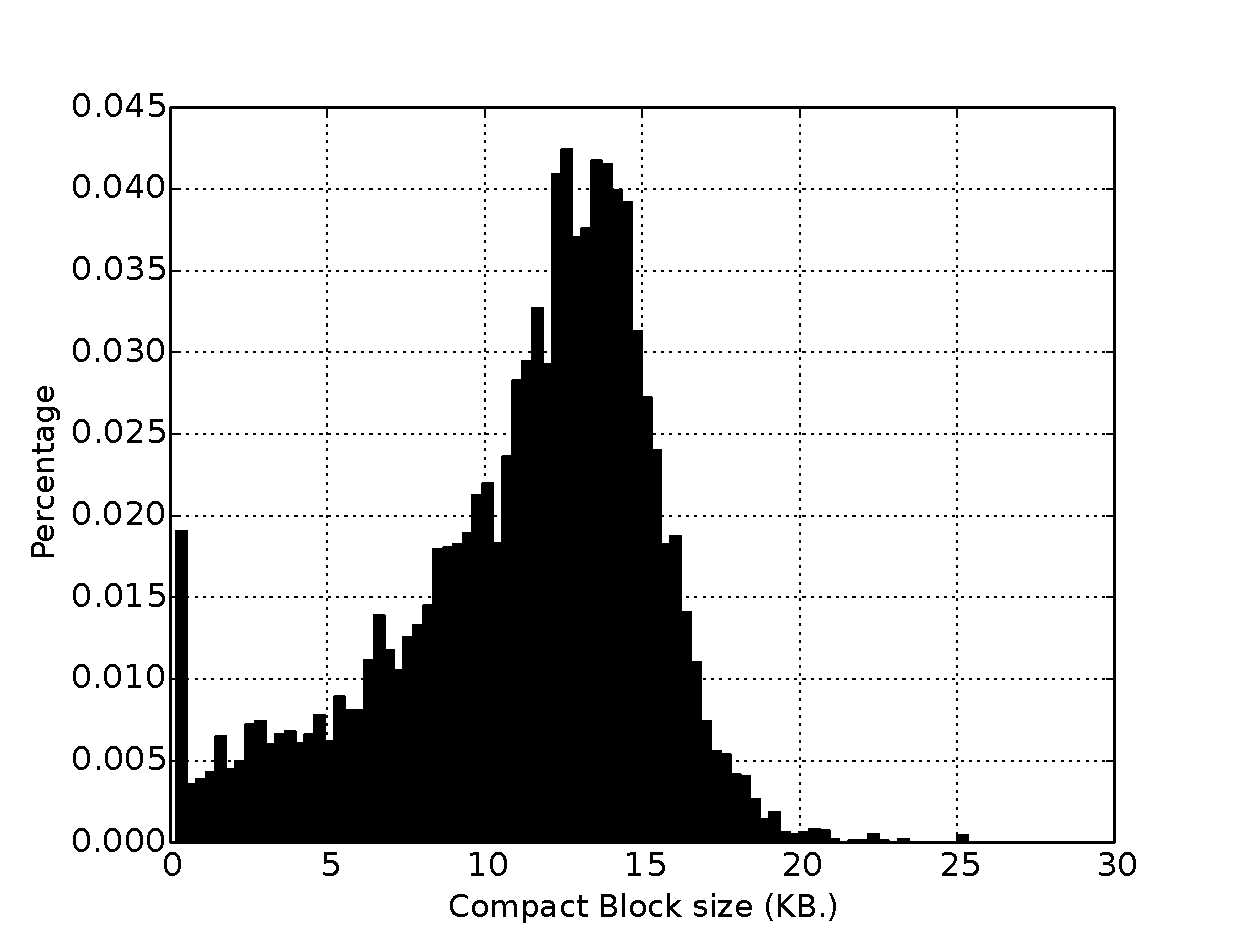
\includegraphics[scale=0.4]{image/cmpctblock_traffic_volume.eps}
\caption{}
\label{fig:cmpctblock_traffic_volume}
\end{figure}
\par In window-based correlation we are looking for the 1 MB spikes in the traffic. However, in the compact blocks, full blocks traffic volume (1 MB) are just transmitted if the receiving node doesn't share any transaction in the mempool, which is a rare case. \shahrzad{my understandings!} So, we should change the $window \ size$ which is $\frac{block\ size}{BW} + delta$. We don't consider $\frac{block\ size}{BW}$ and only consider $delta$ in the worst case which is the block propagation delay that we are waiting for a block. The threshold defined in the window-based correlation scheme will be changed from $block\ size \pm traffic \ std $ to a range between $50$ to $200 \ KB$. 
\par Figure  \ref{fig:cmpct_btc_comparison} shows the comparison between window-based correlation scheme and statistical correlation scheme. AS we can see in figure \ref{fig:cmpct_btc_comparison} window-based doesn't work in the compact block proposal which is due to the fact that we don't have the high spikes in the traffic as before. \shahrzad{The experiment for window-based scheme needs to be rerun.}
\begin{figure}
\centering
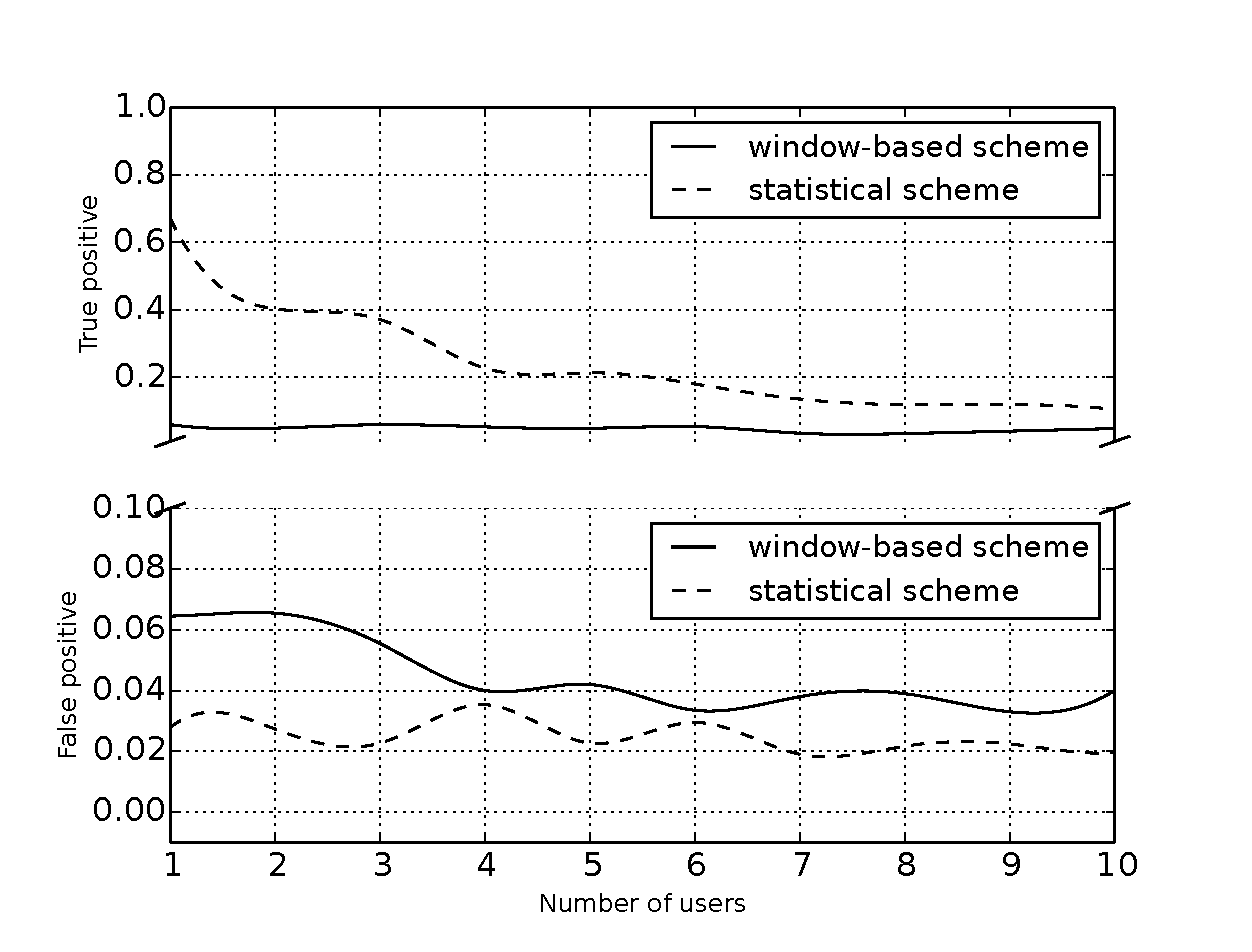
\includegraphics[scale=0.4]{image/cmpct_btc_comparison.eps}
\caption{Comparison between window-based correlation scheme and statistical correlation scheme}
\label{fig:cmpct_btc_comparison}
\end{figure}

\subsubsection{Packet Size Analysis}
\par We capture traffic of Bitcoin for 31 days for the compact block version. Then we measure the number of packets of each message. The histogram of each Bitcoin communication message packet sizes is shown from figure \ref{fig:inv_pktsizes} to figure \ref{}. Figure \ref{fig:aggregate_pkt_size_upstream} and \ref{fig:aggregate_pkt_size_downstream} shows the histogram of size of all of the packets. 
\par Table \ref{} shows the packet number of each message and its percentage of all traffic. As said before the results are over 31 days of Bitcoin traffic.
\begin{center}
\begin{tabular}{|c|c|c|} \hline
Message & Number of packets & Proportion \\ \hline
\code{inv} & 7730342 & 27.240\% \\ \hline
\code{getdata} & 587599 & 2.070\% \\ \hline
\code{block} & 93868 & 0.330 \% \\ \hline
\code{sendcmpct} & 71838 & 0.253\% \\ \hline
\code{cmpctblock} & 90548 & 0.319\% \\ \hline
\code{getblocktxn} & 1132 & 0.003 \% \\ \hline
\code{blocktxn} & 34524 & 0.121\% \\ \hline
\code{tx} & 12397851 & 43.688\% \\ \hline
\textbf{Total Number of packets} & 28377838 & 100\%\\ \hline
\end{tabular}
\end{center}


\begin{figure}
\centering
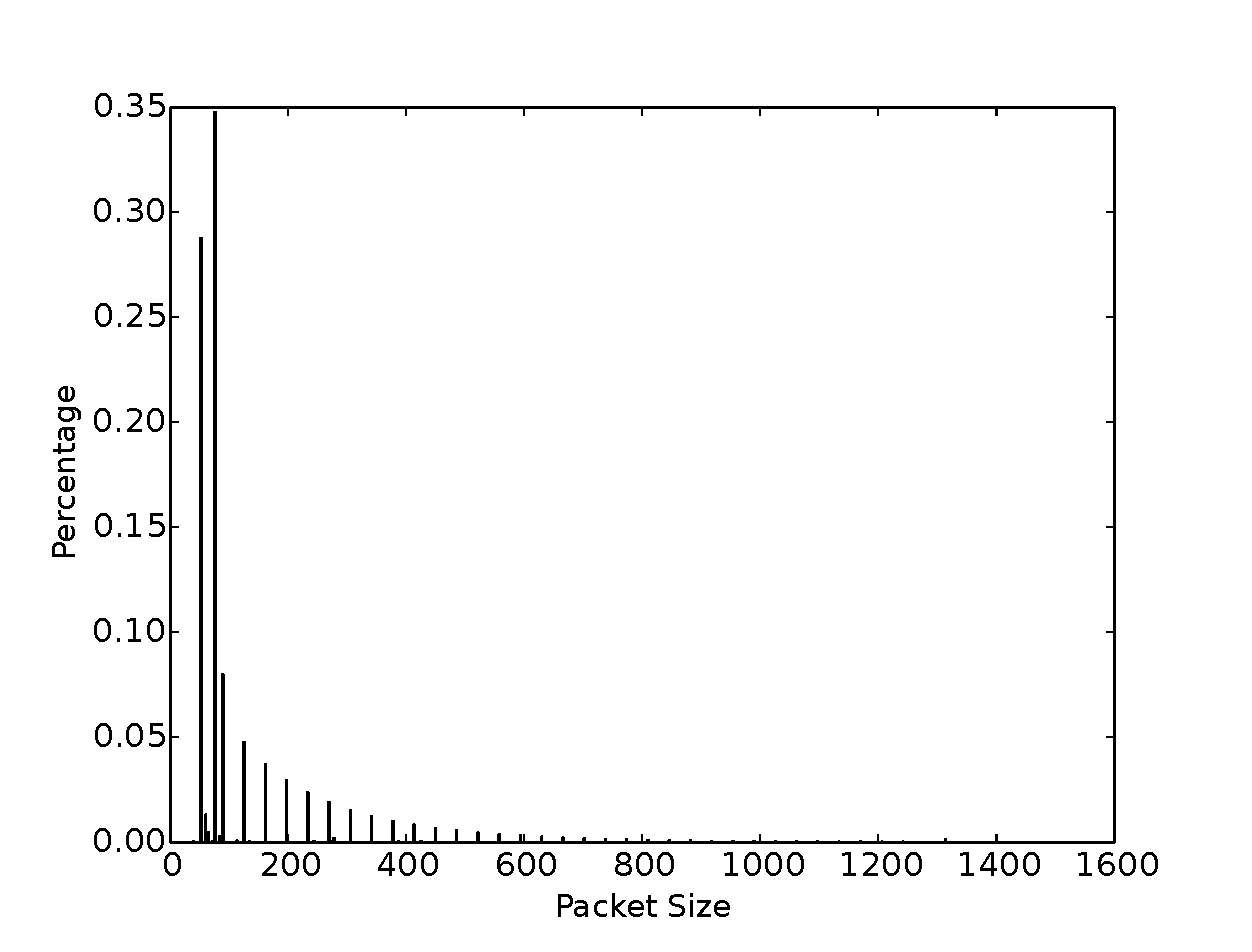
\includegraphics[scale=0.4]{image/cmpctblock_pkt_size_upstream.eps}
\caption{Distribution of packet sizes in a upstream Bitcoin flow }
\label{fig:aggregate_pkt_size_upstream}
\end{figure}


\begin{figure}
\centering
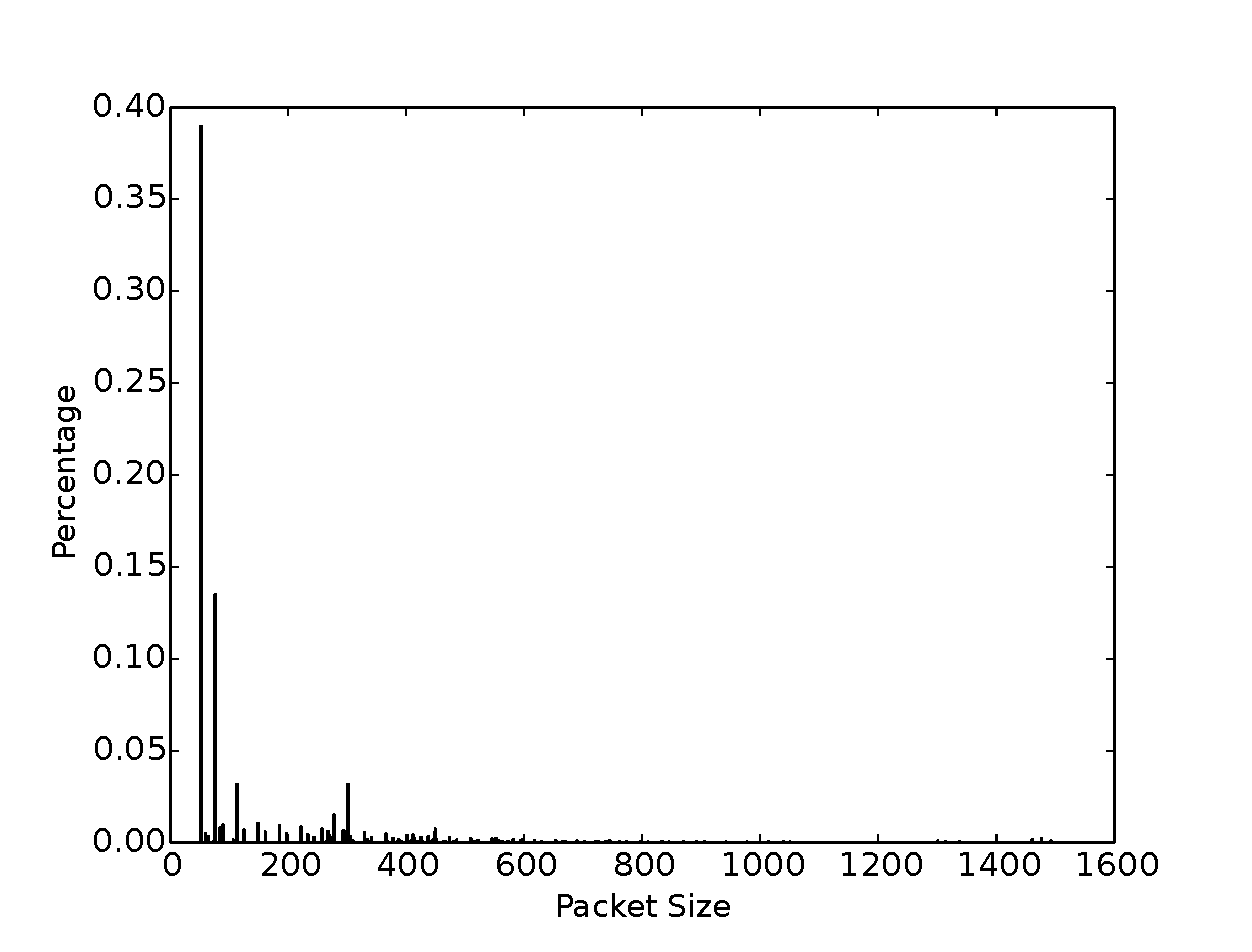
\includegraphics[scale=0.4]{image/cmpctblock_pkt_size_downstream.eps}
\caption{Distribution of packet sizes in a downstream Bitcoin flow }
\label{fig:aggregate_pkt_size_downstream}
\end{figure}


\begin{figure}
\centering
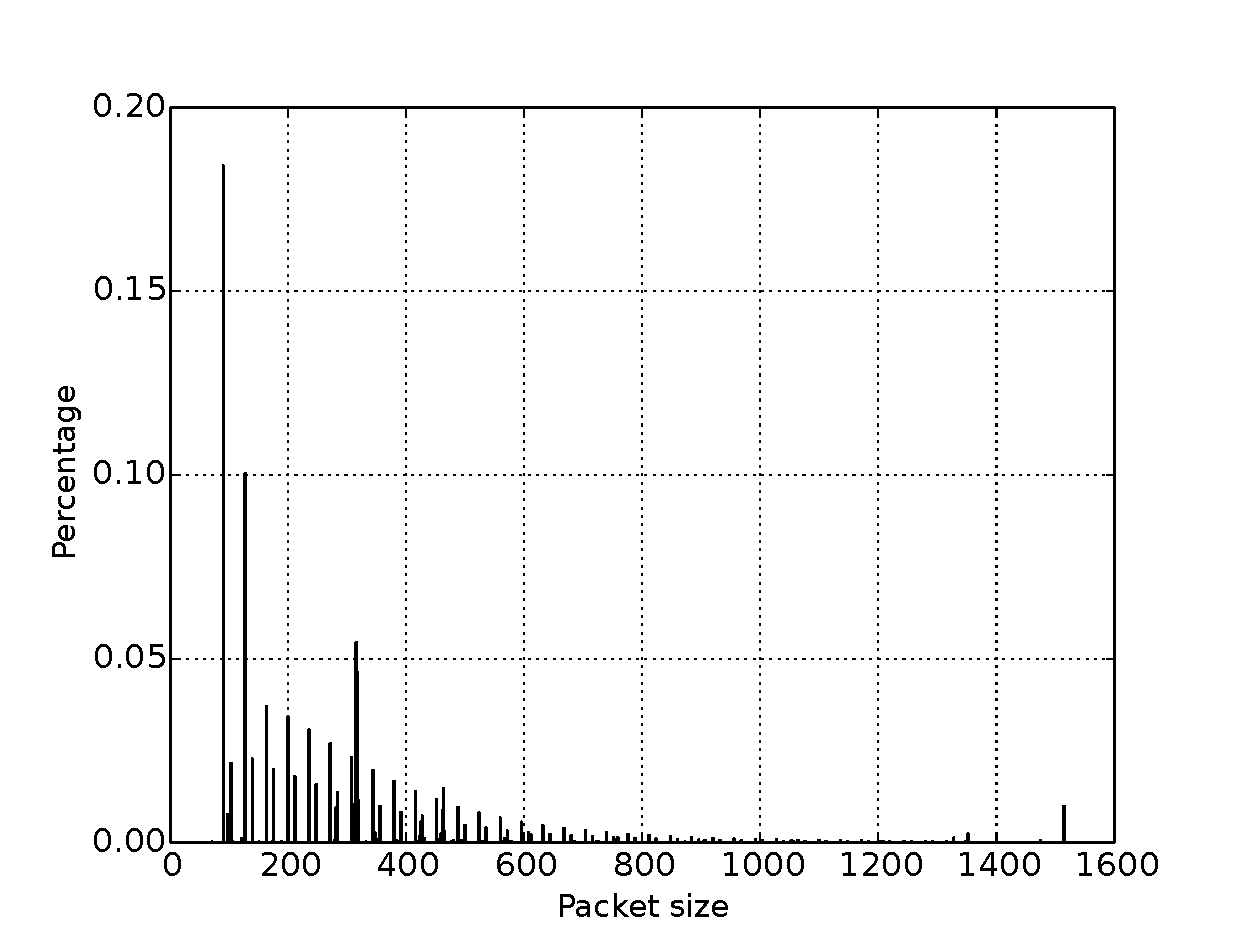
\includegraphics[scale=0.4]{image/inv_pktsizes.eps}
\caption{Distribution of \code{inv} packet sizes}
\label{fig:inv_pktsizes}
\end{figure}

\begin{figure}
\centering
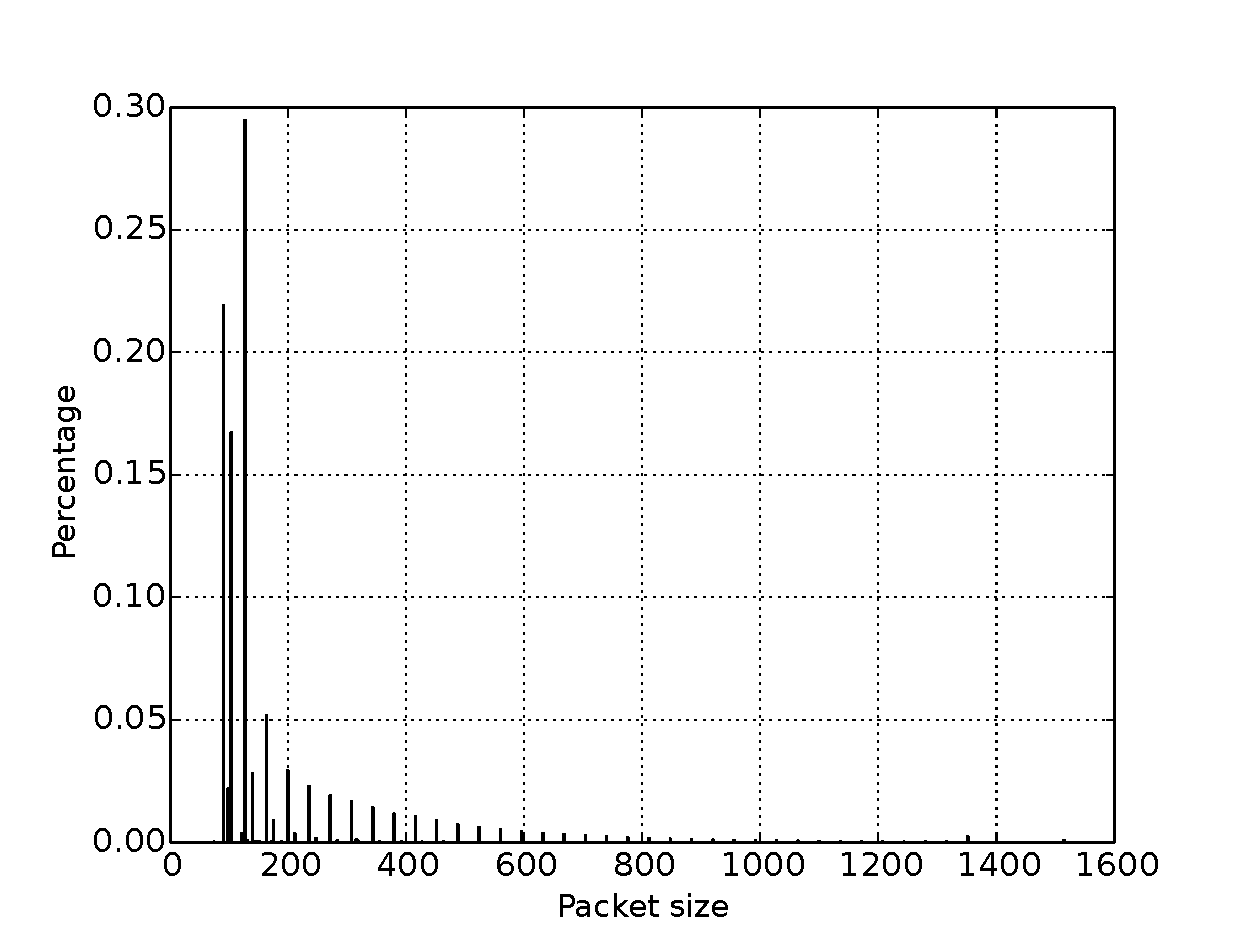
\includegraphics[scale=0.4]{image/getdata_pktsizes.eps}
\caption{Distribution of \code{getdata} packet sizes}
\label{fig:getdata_pktsizes}
\end{figure}


\begin{figure}
\centering
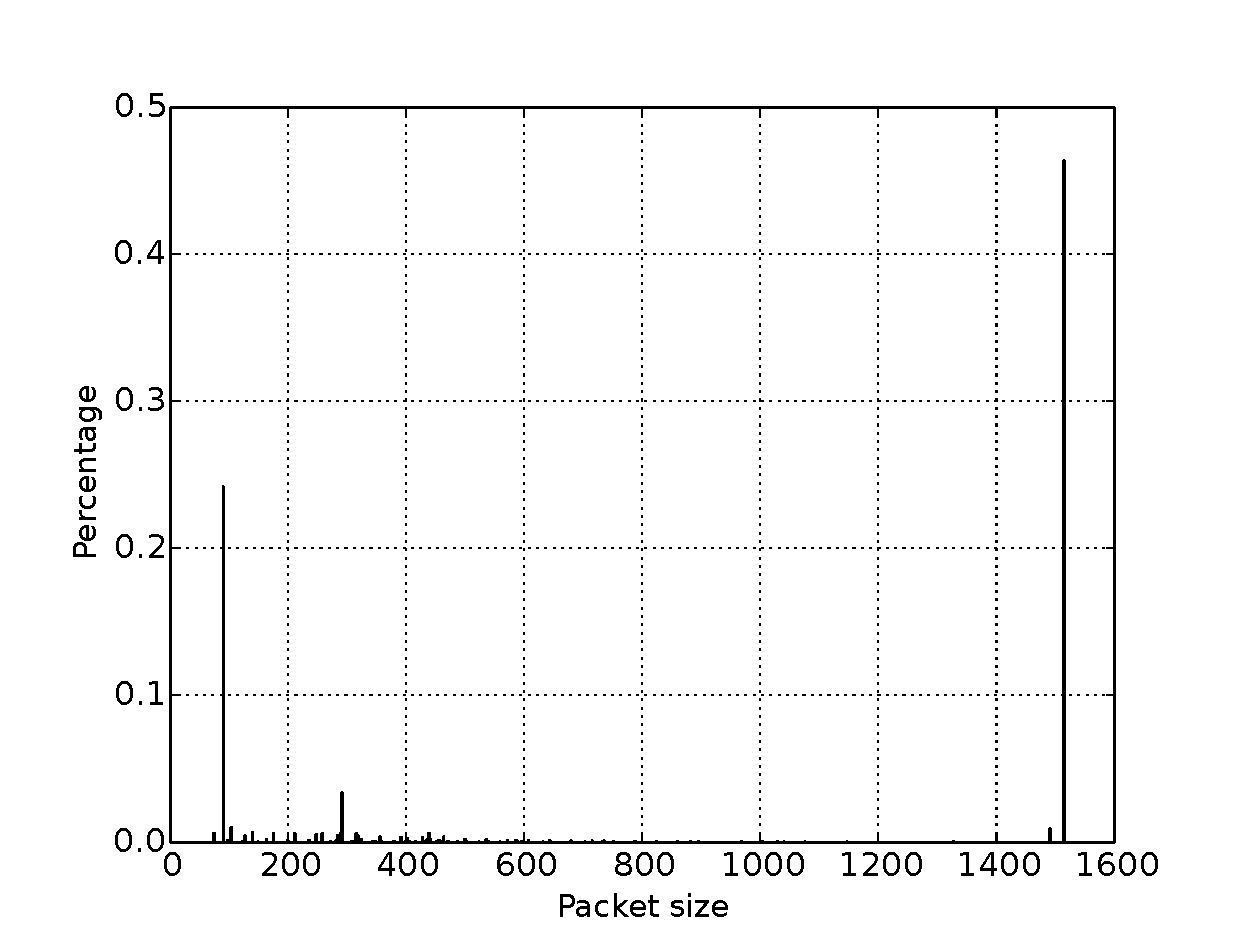
\includegraphics[scale=0.4]{image/block_pktsizes.eps}
\caption{Distribution of \code{block} packet sizes}
\label{fig:block_pktsizes}
\end{figure}

\begin{figure}
\centering
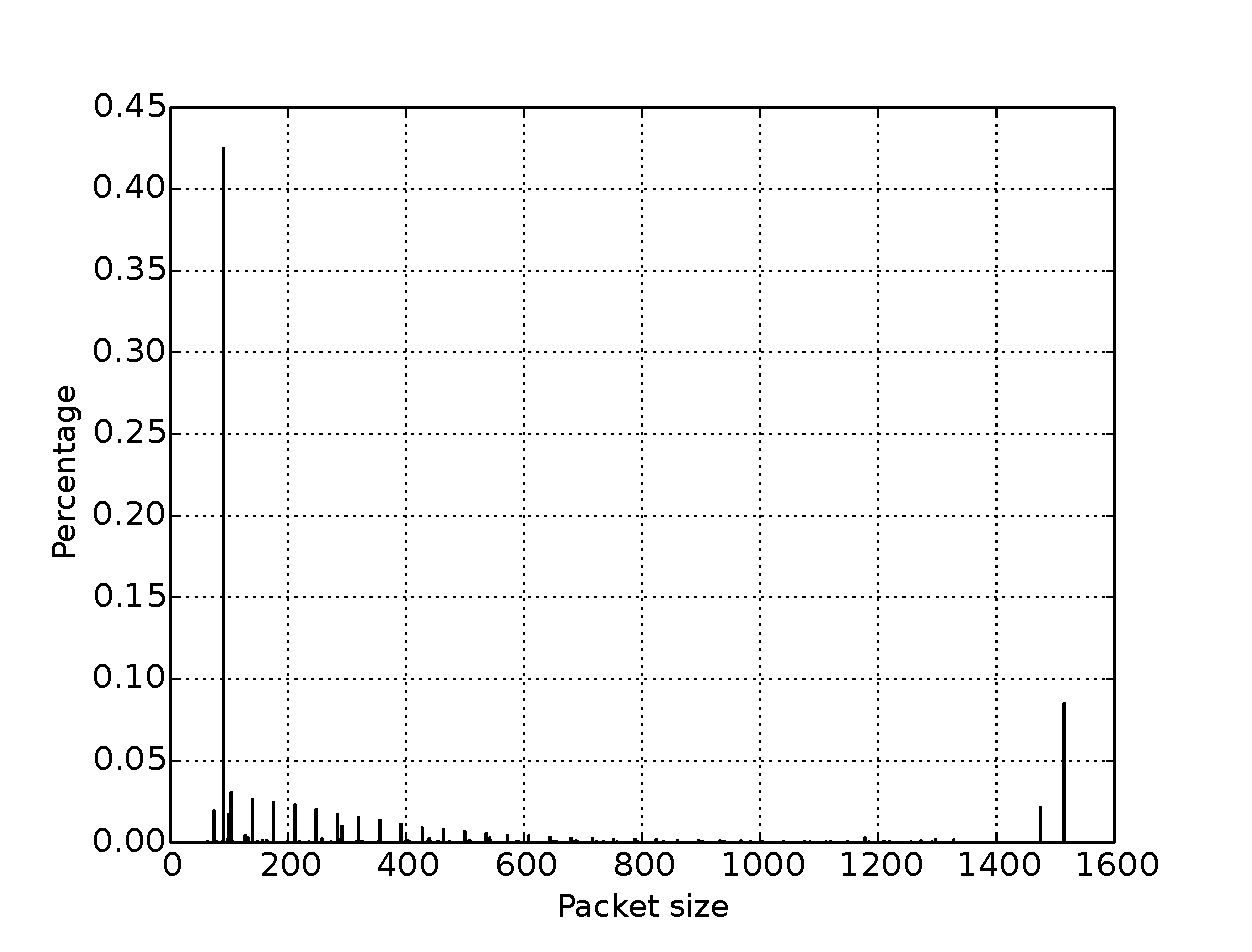
\includegraphics[scale=0.4]{image/sendcmpct_pktsizes.eps}
\caption{Distribution of \code{sendcmpct} packet sizes}
\label{fig:sendcmpct_pktsizes}
\end{figure}

\begin{figure}
\centering
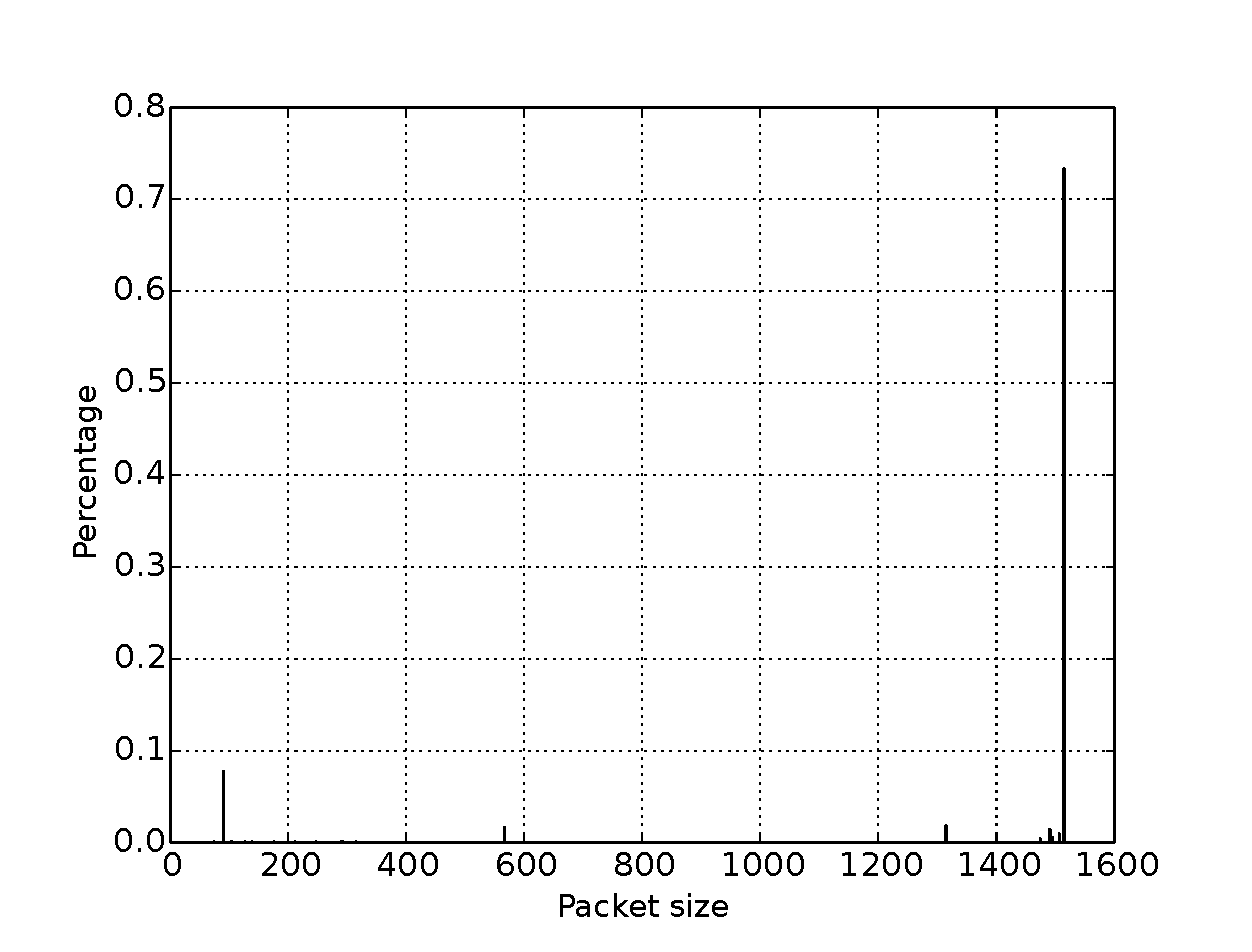
\includegraphics[scale=0.4]{image/cmpctblock_pktsizes.eps}
\caption{Distribution of \code{cmpctblock} packet sizes}
\label{fig:cmpctblock_pktsizes}
\end{figure}

\begin{figure}
\centering
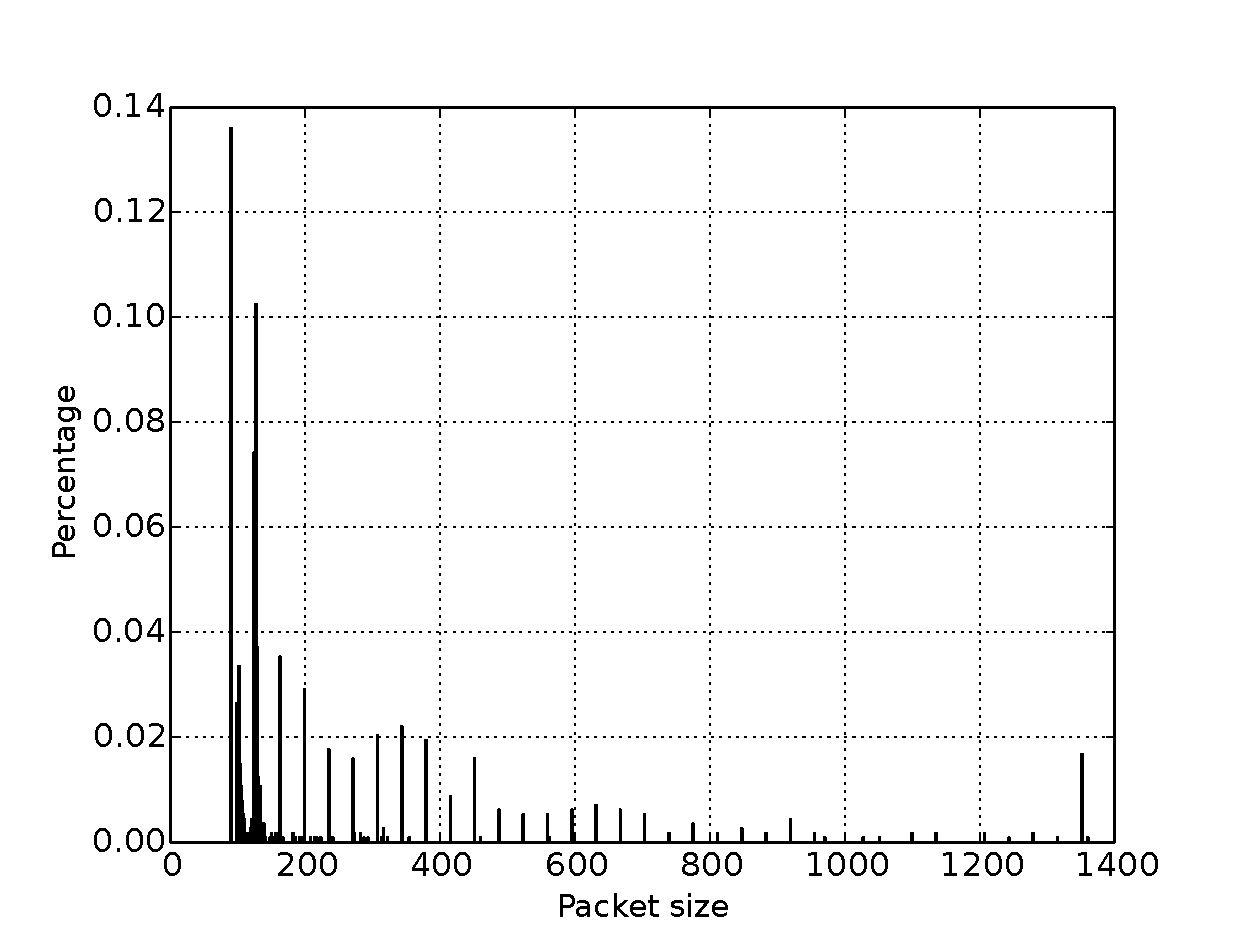
\includegraphics[scale=0.4]{image/getblocktxn_pktsizes.eps}
\caption{Distribution of \code{getblocktxn} packet sizes}
\label{fig:getblocktxn_pktsizes}
\end{figure}

\begin{figure}
\centering
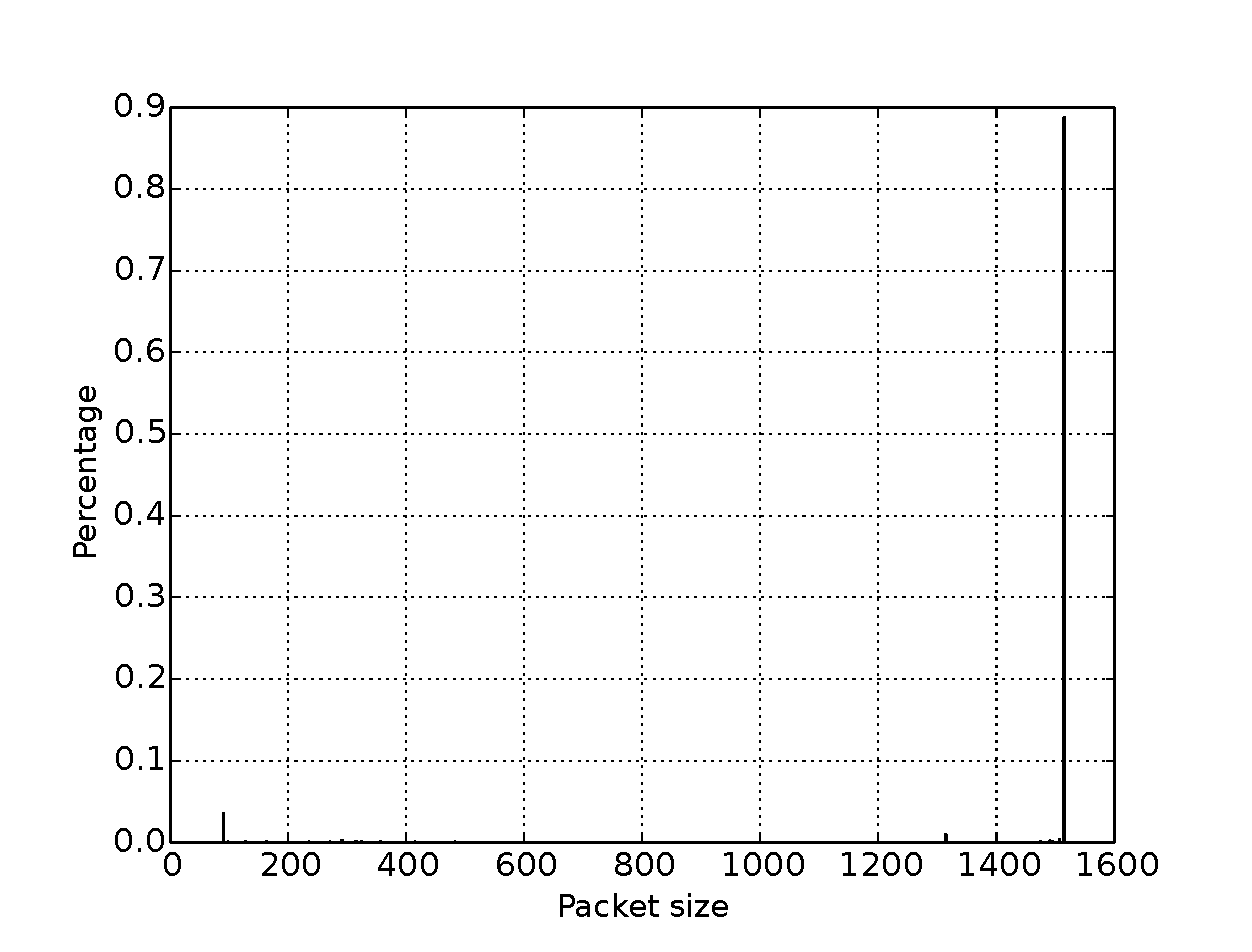
\includegraphics[scale=0.4]{image/blocktxn_pktsizes.eps}
\caption{Distribution of \code{blocktxn} packet sizes}
\label{fig:blocktxn_pktsizes}
\end{figure}


\begin{figure}
\centering
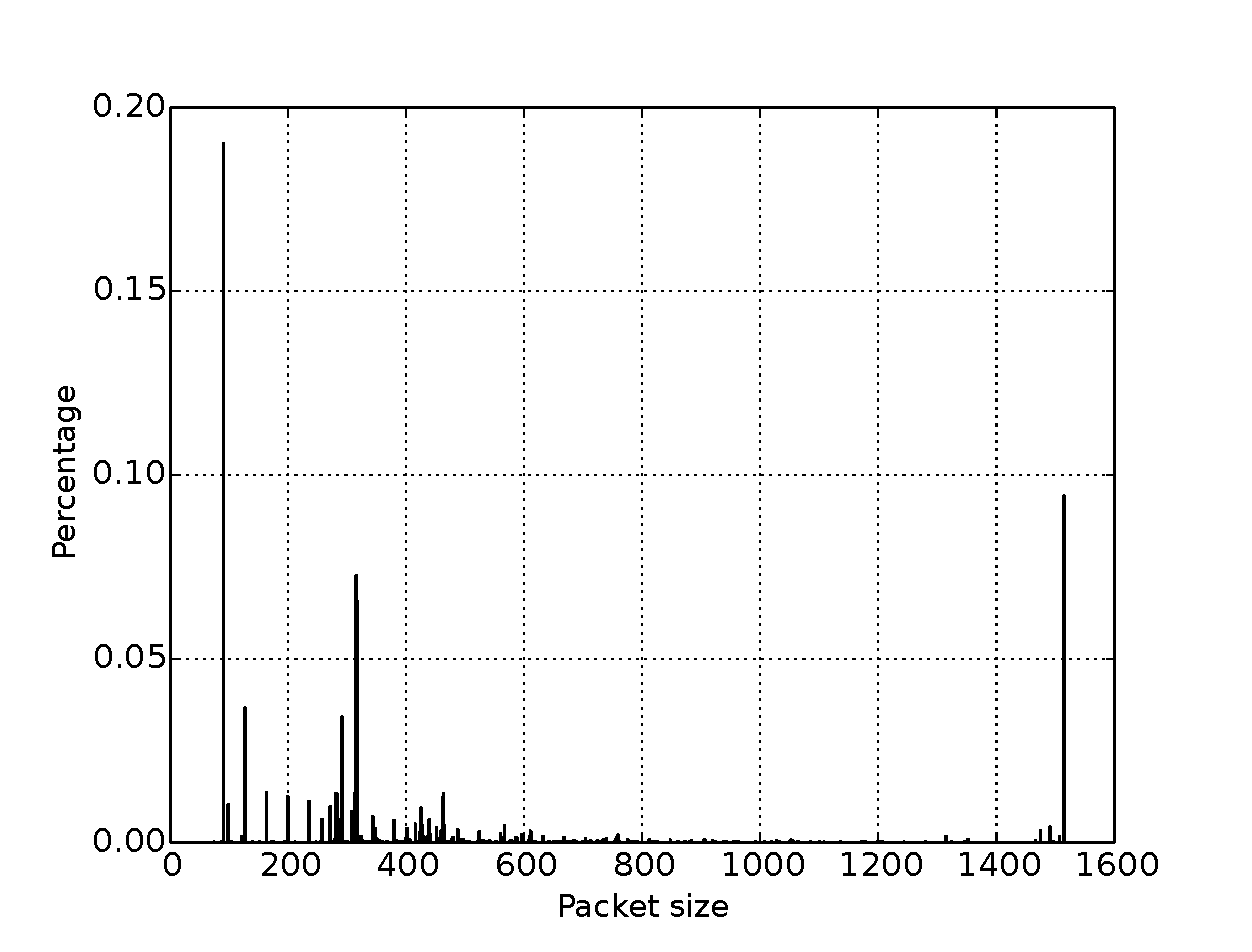
\includegraphics[scale=0.4]{image/tx_pktsizes.eps}
\caption{Distribution of \code{tx} packet sizes}
\label{fig:tx_pktsizes}
\end{figure}


\begin{figure}
\centering
\includegraphics[scale=0.4]{image/reg_traffic_pkt_size.eps}
\caption{Distribution of packet sizes in a regular traffic flow}
\label{fig:reg_traffic_pkt_size}
\end{figure}